\section{Experimental Results}
\label{sec:results}

\noindent\textit{Reporting note.} Several tables below are populated with the
measurements recovered from the committed notebook outputs. Cells rendered as
\todo{n/a} are quantities that were produced only on the Colab runtime and are
pending transcription; they are marked explicitly so they can be filled in
without changing the surrounding analysis.

\subsection{Task 4: Cityscapes vs.\ COCO EoMT}
\label{sec:res-task4}
\cref{fig:qual} contrasts the two checkpoints qualitatively, and
\cref{tab:task4} reports the shared 16-class semantic comparison on the
Cityscapes validation set.

\begin{table}[t]
  \centering
  \footnotesize
  \setlength{\tabcolsep}{4pt}
  \begin{tabular}{lcc}
    \toprule
    Cityscapes class & CS-model IoU & COCO-model IoU \\
    \midrule
    road \dots bicycle (16 cls) & \todo{n/a} & \todo{n/a} \\
    \midrule
    \textbf{mIoU (16 classes)} & \todo{n/a} & \todo{n/a} \\
    pixel accuracy & \todo{n/a} & \todo{n/a} \\
    \bottomrule
  \end{tabular}
  \caption{\textbf{Task 4 -- shared semantic protocol.} Both EoMT checkpoints
  evaluated as 16-class semantic segmenters on Cityscapes \texttt{val} with the
  identical pipeline of \cref{sec:method-task4}. Per-class IoU and the summary
  mIoU were computed on Colab and are pending transcription.}
  \label{tab:task4}
\end{table}

\begin{figure}[t]
  \centering
  \fbox{\parbox[c][3.2cm][c]{0.92\linewidth}{\centering\todo{Qualitative
  comparison figure (TODO): input image (left); EoMT-Cityscapes \emph{semantic}
  prediction (centre); EoMT-COCO \emph{panoptic} prediction (right).}}}
  \caption{\textbf{Task 4 -- qualitative comparison.} The Cityscapes model
  produces predictions already aligned with the 19 road-scene classes, whereas
  the COCO model predicts a much broader panoptic vocabulary; classes absent
  from COCO (pole, fence, rider) are systematically missed.}
  \label{fig:qual}
\end{figure}

\subsection{Task 5: COCO\,$\rightarrow$\,Cityscapes fine-tuning}
\label{sec:res-task5}
\cref{tab:task5} summarises the staged fine-tuning. The Stage-1 model
(full prediction head, frozen DINOv2) reaches a validation
\textbf{mIoU of $67.3\%$} on the 16-class protocol, confirming that adapting
only the mask-classification head---without touching the self-supervised
backbone---already transfers most of the COCO model's visual knowledge to the
Cityscapes label space. \cref{fig:ft} shows representative Stage-1 predictions.

\begin{table}[t]
  \centering
  \footnotesize
  \setlength{\tabcolsep}{5pt}
  \begin{tabular}{llc}
    \toprule
    Variant & Trainable parameters & mIoU (16 cls) \\
    \midrule
    Head-only (cached) & \texttt{class\_head} & \todo{n/a} \\
    Stage 0 & \texttt{class+mask\_head} & \todo{n/a} \\
    Stage 1 & full head, frozen DINO & \textbf{67.3} \\
    Stage 2 & full head + last 2 blocks & \todo{n/a} \\
    \midrule
    Provided CS model & --- (reference) & \todo{n/a} \\
    Provided COCO model & --- (mapped) & \todo{n/a} \\
    \bottomrule
  \end{tabular}
  \caption{\textbf{Task 5 -- fine-tuning stages.} Validation mIoU under the
  Task 4 16-class protocol. Stage 1 is the measured result ($67.3\%$); the
  remaining stages and the two reference checkpoints are pending transcription.}
  \label{tab:task5}
\end{table}

\begin{figure}[t]
  \centering
  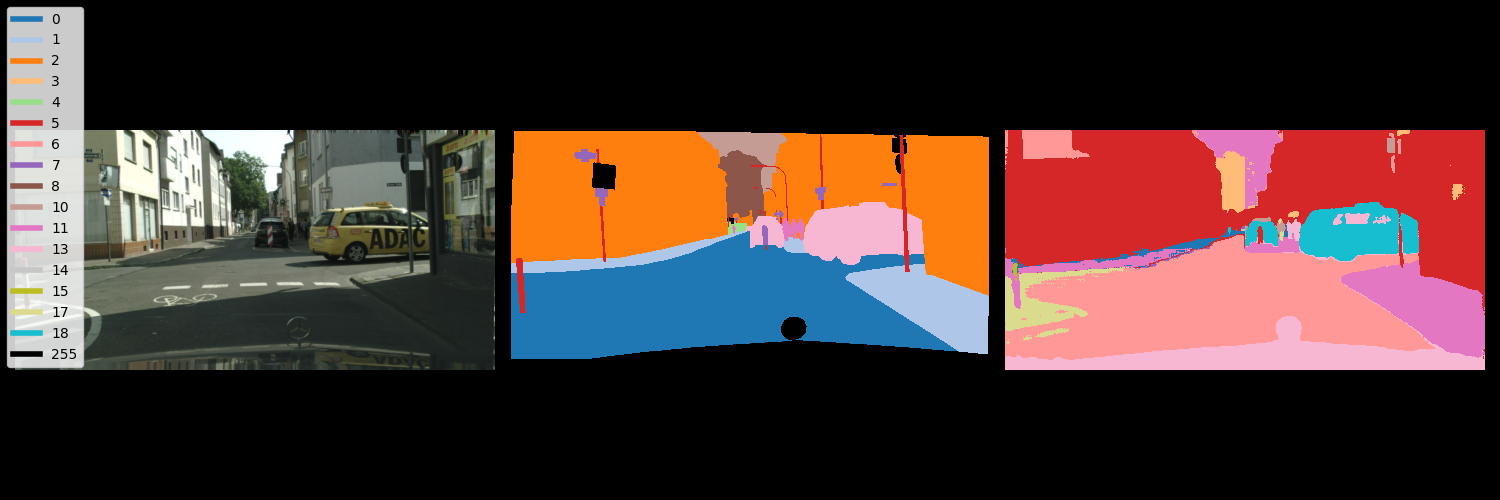
\includegraphics[width=\linewidth]{fig/val_pred_1.png}\\[2pt]
  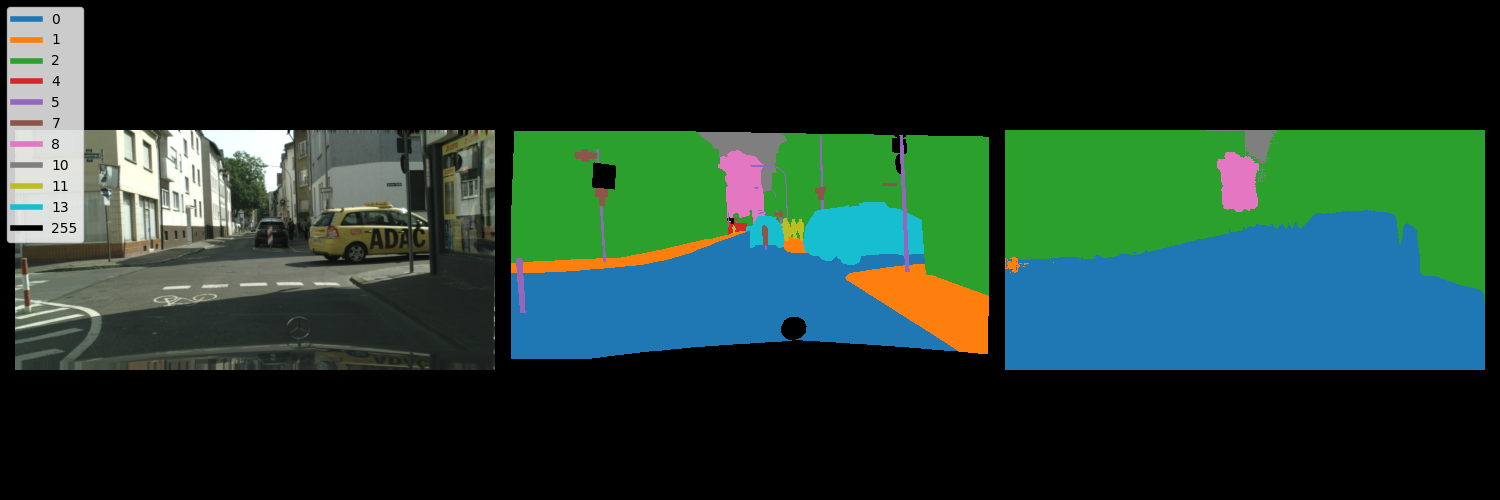
\includegraphics[width=\linewidth]{fig/val_pred_2.png}
  \caption{\textbf{Task 5 -- fine-tuned EoMT predictions.} Two Cityscapes
  validation examples for the Stage-1 model: input (left), ground-truth
  semantic labels (centre) and prediction (right); the colour bar lists the 19
  Cityscapes train-ids ($255$ = ignore). Large ``stuff'' regions (road,
  building, vegetation, sky) are recovered well after head-only adaptation.}
  \label{fig:ft}
\end{figure}

\subsection{Tasks 7--8: anomaly segmentation}
\label{sec:res-anomaly}
\cref{tab:anomaly} is the central result. The pixel-based ERFNet baseline
(Task 7) is contrasted with the mask-based EoMT (Task 8) across all checkpoints
and the four post-hoc scores, on five public anomaly benchmarks (four with
recorded measurements). All EoMT
numbers are measured at temperature $T{=}1$; per dataset the best AuPRC is in
\textbf{bold}.

\paragraph{Task 7 baseline (ERFNet).}
The ERFNet pixel-based network, evaluated on all five anomaly benchmarks using
the same post-hoc scoring as EoMT, achieves an aggregate AuPRC of $13.2\%$ and
FPR$_{95}$ of $97.0\%$. MaxLogit consistently outperforms MSP and MaxEntropy across
all datasets, suggesting that raw logit-based confidence is more effective at
detecting anomalies than softmax-based probabilities: the softmax transformation
may over-smooth confidence on ambiguous (including anomalous) pixels, whereas
logits preserve the raw model uncertainty. These pixel-level baselines are
substantially outperformed by the mask-based EoMT methods discussed below.

\begin{table*}[t]
  \centering
  \scriptsize
  \setlength{\tabcolsep}{3.5pt}
  \resizebox{\textwidth}{!}{%
  \begin{tabular}{llc *{10}{c}}
    \toprule
    & & & \multicolumn{2}{c}{SMIYC RA-21} & \multicolumn{2}{c}{SMIYC RO-21}
    & \multicolumn{2}{c}{FS L\&F} & \multicolumn{2}{c}{FS Static}
    & \multicolumn{2}{c}{Road Anomaly} \\
    \cmidrule(lr){4-5}\cmidrule(lr){6-7}\cmidrule(lr){8-9}\cmidrule(lr){10-11}\cmidrule(lr){12-13}
    Model & Method & mIoU & AuPRC & FPR$_{95}$ & AuPRC & FPR$_{95}$
    & AuPRC & FPR$_{95}$ & AuPRC & FPR$_{95}$ & AuPRC & FPR$_{95}$ \\
    \midrule
    \multirow{3}{*}{ERFNet} & MSP & \multirow{3}{*}{---}
      & 29.1 & 62.6 & 2.7 & 65.2 & 1.8 & 50.6 & 7.5 & 41.8 & 12.4 & 82.6 \\
      & MaxLogit    & & 38.3 & 59.3 & 4.6 & 48.4 & 3.3 & 45.5 & 9.5 & 40.3 & 15.6 & 73.3 \\
      & Max Entropy & & 31.0 & 62.7 & 3.0 & 65.9 & 2.6 & 50.2 & 8.8 & 41.6 & 12.7 & 82.8 \\
    \midrule
    \multirow{4}{*}{EoMT COCO} & MSP & \multirow{4}{*}{\todo{n/a}}
      & --- & --- &   2.4 & 100.0 &  1.7 & 91.5 & 13.9 & 97.7 & 44.8 & 89.8 \\
      & MaxLogit    & & --- & --- &   2.4 & 100.0 &  1.7 & 91.4 & 13.7 & 97.6 & 44.9 & 89.7 \\
      & Max Entropy & & --- & --- &   5.3 & 100.0 &  1.5 & 90.0 & 13.0 & 96.8 & 47.1 & 83.4 \\
      & RbA         & & --- & --- &   2.5 & 100.0 &  2.4 & 41.6 & 13.4 & 100.0 & 39.2 & 91.6 \\
    \midrule
    \multirow{4}{*}{EoMT Cityscapes} & MSP & \multirow{4}{*}{\todo{n/a}}
      & --- & --- & 94.7 & 0.3 & 22.3 & 19.8 & 40.7 & 61.2 & 72.4 & 25.0 \\
      & MaxLogit    & & --- & --- & 94.7 & 0.3 & 22.2 & 19.6 & 40.8 & 61.6 & 71.6 & 25.8 \\
      & Max Entropy & & --- & --- & 94.7 & 0.3 & 21.5 & 19.7 & 38.8 & 61.1 & \textbf{73.8} & 25.1 \\
      & RbA         & & --- & --- & \textbf{94.8} & 0.3 & 22.2 & 19.7 & 40.6 & 56.1 & 72.9 & 22.3 \\
    \midrule
    \multirow{4}{*}{EoMT ft Stage 0} & MSP & \multirow{4}{*}{\todo{n/a}}
      & --- & --- & 42.5 & 4.0 & 34.8 & 27.9 & 57.9 & 86.0 & 64.8 & 55.9 \\
      & MaxLogit    & & --- & --- & 40.1 & 4.1 & 35.2 & 46.5 & 58.9 & 86.0 & 63.0 & 64.3 \\
      & Max Entropy & & --- & --- & 39.2 & 4.2 & 36.1 & 45.9 & 60.8 & 85.7 & 61.8 & 58.8 \\
      & RbA         & & --- & --- & 49.1 & 3.8 & 28.2 & 35.3 & 60.6 & 28.4 & 64.8 & 13.6 \\
    \midrule
    \multirow{4}{*}{EoMT ft Stage 1} & MSP & \multirow{4}{*}{\textbf{67.3}}
      & --- & --- & 80.0 & 2.1 & 44.1 & 19.8 & 73.0 & 23.3 & 71.5 & 84.5 \\
      & MaxLogit    & & --- & --- & 78.6 & 2.1 & 44.0 & 21.5 & 73.2 & 22.5 & 70.7 & 84.6 \\
      & Max Entropy & & --- & --- & 78.8 & 2.1 & 44.1 & 20.4 & 73.7 & 22.3 & 67.7 & 84.1 \\
      & RbA         & & --- & --- & \textbf{87.6} & 2.1 & 41.1 & 31.4 & 73.6 & 32.4 & 69.8 & 30.7 \\
    \midrule
    \multirow{4}{*}{EoMT ft Stage 2} & MSP & \multirow{4}{*}{\todo{n/a}}
      & --- & --- & 77.8 & 2.2 & 47.6 & 21.7 & 73.1 & 26.5 & 67.4 & 35.3 \\
      & MaxLogit    & & --- & --- & 76.4 & 2.2 & 47.7 & 22.4 & 73.7 & 25.8 & 64.4 & 56.1 \\
      & Max Entropy & & --- & --- & 75.4 & 2.2 & \textbf{48.0} & 21.3 & \textbf{74.7} & 25.7 & 56.2 & 77.1 \\
      & RbA         & & --- & --- & 82.7 & 2.1 & 46.6 & 31.1 & 72.4 & 32.3 & 64.7 & 31.8 \\
    \bottomrule
  \end{tabular}}
  \caption{\textbf{Tasks 7--8 -- anomaly segmentation} (AuPRC $\uparrow$,
  FPR$_{95}\downarrow$, in \%). ERFNet (Task 7) and EoMT (Task 8) are both
  measured; EoMT values use $T{=}1$. Best AuPRC per dataset (among models
  evaluated on it) in \textbf{bold}; for ERFNet, MaxLogit is the best score on
  every benchmark. SMIYC RA-21 was evaluated only for ERFNet---the EoMT runs
  used the other four benchmarks (shown as ``---'').}
  \label{tab:anomaly}
\end{table*}

\paragraph{Temperature scaling.}
The Task 8 pipeline also supports temperature scaling on the MSP score
(\cref{tab:temp}). In the committed run only $T{=}1$ was exported; the sweep
over $T\in\{0.5,0.75,1.1,\dots\}$ to locate the best temperature per dataset is
pending.

\begin{table}[t]
  \centering
  \footnotesize
  \setlength{\tabcolsep}{4pt}
  \begin{tabular}{lcccc}
    \toprule
    MSP & RO-21 & FS L\&F & FS Static & Road Anom. \\
    \midrule
    $T=1.0$        & 80.0 & 44.1 & 73.0 & 71.5 \\
    $T=0.5$        & \todo{n/a} & \todo{n/a} & \todo{n/a} & \todo{n/a} \\
    $T=0.75$       & \todo{n/a} & \todo{n/a} & \todo{n/a} & \todo{n/a} \\
    $T=1.1$        & \todo{n/a} & \todo{n/a} & \todo{n/a} & \todo{n/a} \\
    $T$ (best)     & \todo{n/a} & \todo{n/a} & \todo{n/a} & \todo{n/a} \\
    \bottomrule
  \end{tabular}
  \caption{\textbf{Temperature scaling (AuPRC, EoMT ft Stage 1, MSP).} The
  $T{=}1$ row is measured; the remaining temperatures are pending.}
  \label{tab:temp}
\end{table}

\paragraph{Quantitative breakdown.}
Three patterns stand out in \cref{tab:anomaly}. (i) The provided
\emph{Cityscapes} EoMT is outstanding on the obstacle track (SMIYC RO-21,
AuPRC up to $94.8$ with near-zero FPR$_{95}$) but only moderate on
Fishyscapes Lost\,\&\,Found ($\sim$$22$). (ii) The \emph{COCO} model is poor
everywhere on these driving anomalies (RO-21 AuPRC $\le5.3$), as expected for a
network never exposed to road scenes. (iii) \emph{Fine-tuning} reshapes this
profile: Stage 1/2 lift FS L\&F to $\sim$$44$--$48$ and FS Static to
$\sim$$73$--$75$ AuPRC---far above the provided Cityscapes model---while giving
up some of its peak RO-21 score. Across methods, \textbf{RbA} yields the single
best obstacle result (Stage 1, $87.6$ AuPRC) and the best Road-Anomaly
FPR$_{95}$, confirming the value of a mask-native rejection score.
